%! Author = vsharma
%! Date = 25.09.2022
% !TeX spellcheck = en_EN

\chapter{Evaluation}

\par In this chapter, we evaluate the efficiency of Prowler against security vulnerabilities based on the approaches from the previous chapter. The result of the evaluation of each approach is discussed here.

\par In the end, a comparison between the assessment of security vulnerabilities performed using Prowler and
ScoutSuite is also highlighted which showcases the efficiency of each tool individually.

\section{Using Test Driven Approach}
\begin{figure}
    \centering
    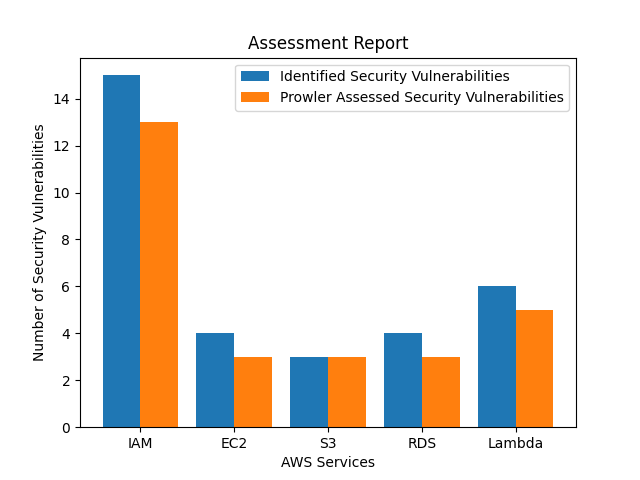
\includegraphics[width=\textwidth]{assessmentgraph.png}
    \caption{Prowler Assessment Graph}
    \label{fig:prowlerefficiency}
\end{figure}

\par The test-driven approach requires developing the test cases for the possible assessable scenario of a check in Prowler that performs the security assessment of an identified security vulnerability in the AWS service. The individual test cases are developed, and their results are noted.

\par The checks corresponding to the identified security vulnerabilities that can be assessed in Prowler are determined. Upon determination of the possible check in Prowler, the test cases are developed. Once all the test scenarios for the different checks in Prowler are developed and verified, the efficiency of Prowler is calculated against the identified security vulnerabilities for individual AWS services. The efficiency calculation is done programmatically.

\par The process for calculating the efficiency of Prowler begins by determining the count of the security
vulnerabilities that are identified for an AWS service. After determining the number of security vulnerabilities that
are identified for the AWS service, the number of security vulnerabilities that are assessed using Prowler for that AWS service is determined. For example, if we consider Amazon RDS, the number of identified security vulnerabilities as seen from the graph \ref{fig:prowlerefficiency} is 4, correspondingly the number of security vulnerabilities that are assessed using Prowler is 3. This process is performed for the 5 AWS services that are chosen for this research work. In the end, it is possible to determine how efficient is Prowler in assessing the security vulnerabilities of each AWS service.

\par The graph \ref{fig:prowlerefficiency} highlights the total number of security vulnerabilities identified for an AWS service and the number of security vulnerabilities that are assessed using Prowler for the AWS service.

\par Starting with IAM, out of the 15 identified security vulnerabilities, 13 of those security vulnerabilities are
assessed using Prowler. The 2 unassessed security using Prowler part of excessive privileges. Excessive privilege is
one of the most common security vulnerabilities that can result in severe security issues such as compromission of
AWS accounts and many more. Excessive privilege can cause an identity to modify its own rights. The identity has all
the permissions it needs to move throughout the environment e.g. make itself an administrator or one identity can
modify another identity’s credentials to impersonate it. For example, identity has permission to modify roles in AWS.
While this identity is unable to read sensitive data itself, it can modify other roles so that it can read that data,
and then jump into this new role and reach its goal ultimately. Excessive privilege can also occur when an identity
has permission to change the configuration settings on a resource to allow the identity to perform unintended actions
on that resource.

\par Like IAM, looking at the graph for EC2 it can be determined that out of the 4 identified security vulnerabilities, 3 of those security vulnerabilities are assessed using Prowler.  The unassessed security vulnerability using Prowler is the Denial of wallet. Most of the time data loss incidents make the news, but the denial of wallet is one of the common ways that can be found out about a compromise through the AWS bill. Such security vulnerability prevents the system from providing services to legitimate users and is used for the personal gain of the attacker, but it is possible that an attacker just wants to bring hurt the organization.

\par Prowler shows 100 \% efficiency in assessing the security vulnerabilities that are identified in S3 and thus Prowler is highly efficient in performing the security best practices assessments, audits, and incident response for S3.

\par Similar to IAM and EC2, Prowler is able to assess 3 out of the 4 identified security vulnerabilities in RDS. Resources running in an AWS classic resource are not assessable using Prowler. The EC2-Classic platform is retired by Amazon.

\par As seen from the graph \ref{fig:prowlerefficiency}, out of the 6 security vulnerabilities identified in AWS lambda, Prowler can perform the assessment of 5 security vulnerabilities. The unassessed security vulnerability ‘Poisoning of well’ can be highly hazardous where the malicious users inject fake training data with the aim of corrupting the learned model and can spread, affecting the products that draw from it.

\section{Using Open-Source Application}

\begin{figure}
    \centering
    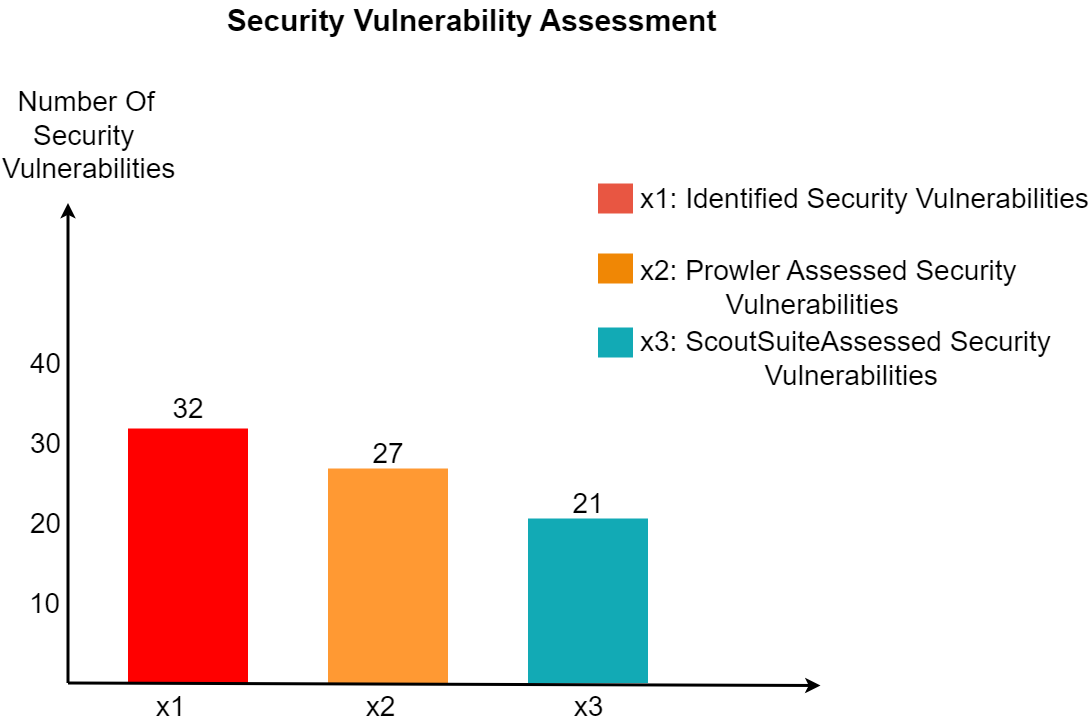
\includegraphics[width=\textwidth]{prowlervsscoutsuite.png}
    \caption{Security Vulnerabilities Assessment Graph}
    \label{fig:prowlervsscoutsuite}
\end{figure}

\par The employee management web application leverages different AWS services namely IAM, EC2, S3, RDS, and Lambda for its deployment on AWS cloud infrastructure as shown in the figure \ref{fig:infrastructure_architecture}. Once the application is deployed on the AWS cloud, the application functionality is verified. The application provides different functions such as adding, updating and deleting the organization’s employee information. The application employs different AWS services for its deployment, thus there could be a chance of introduction of security vulnerability due to misconfiguration or security flaws within the application. In order to deal with these issues, the AWS account must be assessed using the assessment tools against any security vulnerability that might have been introduced while deploying the application on the AWS infrastructure.

\par To assess the AWS account against any security vulnerabilities two security assessment tools namely Prowler and ScoutSuite were introduced in chapter 4. To begin the assessment of the AWS account using Prowler the command \textit{./prowler} is executed, on the other hand, the assessment of security vulnerabilities using ScoutSuite is performed by executing the command \textit{scout aws} is executed.

\par Once the assessment of the AWS account finishes, the assessment report is generated. Prowler supports the generation of assessment reports in multiple formats such as text, mono, CSV, JSON, JSON-ASFF, JUnit-XML, and HTML. This assessment report provides a detailed description of the assessment such as the check in Prowler used to assess a security vulnerability, the severity of the security vulnerability, region, associated AWS service, the result of executing the check, etc. Upon completion of the assessment, ScoutSuite generates the assessment report in PDF format. The assessment report provides a descriptive view of the different AWS services, the resources leveraged by each service, the rules available for each service, etc.

\par Looking at the graph \ref{fig:prowlervsscoutsuite}, it can be seen a total of 32 security vulnerabilities are identified in the five AWS services namely IAM, EC2, S3, RDS, and Lambda. After the assessment of the AWS account finishes, a total of 27 of the identified security vulnerabilities are assessed using Prowler. There are 5 security vulnerabilities that could not be assessed using Prowler as Prowler does not provide checks to assess those 5 security vulnerabilities. Similarly, out of the 32 identified security vulnerabilities, ScoutSuite can perform the security assessment of 21 security vulnerabilities. There are 11 security vulnerabilities that are not assessed using the rules provided by ScoutSuite.

\par Based on the assessment of security vulnerabilities performed using the two security tools, it is possible to calculate the efficiency of the tools. The formula to calculate efficiency of the two security assessment tools mathematically is the ratio of output to input expressed as a percentage \cite{88}. Using this formula, the overall percentage efficiency of Prowler is calculated to be 84 \% and the overall efficiency of ScoutSuite is calculated to be 65 \%.

\par Prowler boasts a number of checks that other tools miss, has thorough and considered documentation, and is a reliavle and lightweight piece of software.

\section{Comparision between Prowler and ScoutSuite}

\par Cloud service providers make tools available to secure the cloud systems, but it is ultimately the user’s responsibility to use them.
The control needed to define and implement the cloud infrastructure differs greatly from the controls used in on-premises environments.
Simply transforming the hardware servers to AWS EC2 instances won't make them secure by default.
This is because, while AWS is responsible for the security of the cloud, users are responsible for the security in the cloud.
Due to this, many companies suffer from misconfigured and poorly architected cloud infrastructure, leading to embarrassing data leaks \cite{74}.

\par There are a limited number of tools provided by cloud service providers.
For instance, AWS Security Hub only supports Center for Internet Security (CIS) and Payment Card Industry Data
Security Standard (PCI DSS) benchmarks.
Even that is limited since it cannot produce results on "monitoring" related CIS benchmarks (Section 3).
This is where third-party solutions come in handy \cite{74}.

\par This section shows the assessment of security vulnerability performed using two open-source cloud security assessment tools namely Prowler and ScoutSuite which can help strengthen the cloud security posture without breaking the bank.
In the end, a comparison between the assessment performed using Prowler and ScoutSuite against the different security vulnerabilities identified earlier is highlighted in the table \ref{tab:comparisionresultprowlervsscoutsuite}.

\par This section shows the comparison of the assessment of security vulnerability performed using two open-source cloud security assessment tools namely Prowler and ScoutSuite.
These tools help strengthen the cloud security posture without breaking the bank.
The table \ref{tab:comparisionresultprowlervsscoutsuite} highlights the result of the assessment obtained using the two tools.

\par Assessmement Process:


\par Prowler: Prowler users AWS CLI. Before running Prowler, the AWS CLI must be properly configured with a valid Access Key and Region or declare AWS variables properly.
This can be done by running the command \textit{aws configure}.
The credentials configured in the AWS CLI must be associated with a user.
In order to run all the Prowler checks, managed policies \textit{SecurityAudit} and \textit{ViewOnlyAccess} must be added to the user \cite{75}.

\begin{table}[h!]
    \begin{center}
        \caption{Prowler Extra78}
        \label{tab:prowlerextra}
        \begin{tabular}{|p{1.4cm}|p{1.7cm}|p{1.5cm}|p{4.0cm}|p{5.0cm}|}
            \hline
            \textbf{Result} & \textbf{Severity} & \textbf{CheckID} & \textbf{Check Title} & \textbf{Check Output}\\
            \hline
            Pass & Critical & 7.8 & [extra78] Ensure there are no Public Accessible RDS instances &
            No Publicly Accessible RDS instances found\\
            \hline
        \end{tabular}
    \end{center}
\end{table}

\par The assessment of security vulnerability using Prowler is performed by executing the command \textit{./prowler}.
When the command is run, Prowler authenticates the configured environment variable.
Upon successful authentication, the checks are run over all the AWS regions.
To limit the assessment to a custom profile and region, the command \textit{./prowler -p custom-profile -r us-east-1} is used.
Prowler also enables assessing a single security vulnerability by running the command \textit{./prowler -c check78}.
The check78 is a check id, this check ensures there are no Public Accessible RDS instances (verifies publicly accessible RDS instances).
Table \ref{tab:prowlerextra} shows the execution result of the assessment performed using Prowler \cite{75}.

\par If the user wants to save the assessment report for later analysis, Prowler enables saving the result in different formats such as CSV, JSON, Html, etc.
This is achieved by using the command \textit{./prowler -M csv}\cite{75}.


\par Scout Suite works on machines used to make AWS API calls, such as AWS CLI, EC2 instances, or any other tool based on AWS official SDKs. Similar to Prowler, before starting the assessment AWS CLI must be configured.
AWS CLI can be configured by running the \textit{aws configure} command.
The user credentials configured must be assigned the ReadOnlyAccess and SecurityAudit AWS Managed Policies \cite{76}.

\begin{table}[h!]
    \begin{center}
        \caption{ScoutSuite Publicly accessible RDS instances}
        \label{tab:scoutsuiterule}
        \begin{tabular}{|p{1.4cm}|p{1.7cm}|p{5.0cm}|p{6.0cm}|}
            \hline
            \textbf{Result} & \textbf{Severity} & \textbf{Rule} & \textbf{Rule Title}\\
            \hline
            Good & Danger & rds-instance-publicly-accessible & RDS Instance publicly accessible \\
            \hline
        \end{tabular}
    \end{center}
\end{table}

Once the AWS CLI environment is configured and appropriate credentials are set up, the assessment can be started with ScoutSuite.
If the user wishes to use Scoutsuite against a specific AWS IAM role, the command \textit{scout aws --profile my-aws-cli-profile} is executed.
The assessment is started by executing the command \textit{scout aws}.
ScoutSuite gathers data from APIs, performs the authenticity of the configured environment variable, and pulls info on the cloud services and various resources.
Once Scout Suite finishes auditing the environment, an HTML report will be generated \cite{77}.

Unlike checks in Prowler, ScoutSuite has rules.
To verify publicly accessible RDS instances, ScoutSuite uses the rule \textit{rds-instance-publicly-accessible}.
The result is demonstrated in table \ref{tab:scoutsuiterule} \cite{77}.






\begin{longtable}{|p{10cm}|p{2.2cm}|p{2.2cm}|}
    \hline
    \textbf{Security Vulnerabilities} & \textbf{Prowler} & \textbf{ScoutSuite}\\
    \hline
    Avoid the use of the root account & {{\color{green}\checkmark}} & {{\color{green}\checkmark}} \\
    \hline
    MFA is enabled for all IAM users & {{\color{green}\checkmark}} & {{\color{green}\checkmark}} \\
    \hline
    Credentials unused for 90 days or greater are disabled & {{\color{green}\checkmark}} & {{\color{green}\checkmark}} \\
    \hline
    Access keys are rotated every 90 days or less & {{\color{green}\checkmark}} & {{\color{green}\checkmark}} \\
    \hline
    IAM password policy requires at least one uppercase letter & {{\color{green}\checkmark}} & {{\color{green}\checkmark}} \\
    \hline
    IAM password policy requires at least one lowercase letter & {{\color{green}\checkmark}} & {{\color{green}\checkmark}} \\
    \hline
    IAM password policy requires at least one symbol & {{\color{green}\checkmark}} & {{\color{green}\checkmark}} \\
    \hline
    IAM password policy requires at least one number & {{\color{green}\checkmark}} & {{\color{green}\checkmark}} \\
    \hline
    IAM password policy requires a minimum length of 14 or greater & {{\color{green}\checkmark}} & {{\color{green}\checkmark}} \\
    \hline
    IAM password policy prevents password reuse & {{\color{green}\checkmark}} & {{\color{green}\checkmark}} \\
    \hline
    IAM password policy expires passwords within 90 days or less & {{\color{green}\checkmark}} & {{\color{green}\checkmark}} \\
    \hline
    Password expiration requires an administrator reset &  & \\
    \hline
    Allow users to change their own password &  & \\
    \hline
    Insider Threat & {{\color{green}\checkmark}} & {{\color{green}\checkmark}} \\
    \hline
    Access key for the root account & {{\color{green}\checkmark}} & {{\color{green}\checkmark}} \\
    \hline
    Instances created from Malicious AMI & {{\color{green}\checkmark}} & {{\color{green}\checkmark}} \\
    \hline
    User data public exposure & {{\color{green}\checkmark}} & {{\color{green}\checkmark}} \\
    \hline
    Server-Side Request Forgery & {{\color{green}\checkmark}} &  \\
    \hline
    Denial of Wallet &  & \\
    \hline
    Public exposure of S3 buckets & {{\color{green}\checkmark}} & {{\color{green}\checkmark}} \\
    \hline
    Unencrypted S3 buckets & {{\color{green}\checkmark}} & {{\color{green}\checkmark}} \\
    \hline
    Write access on S3 buckets (Ghostwriter) & {{\color{green}\checkmark}} & {{\color{green}\checkmark}} \\
    \hline
    Publicly accessible RDS instances & {{\color{green}\checkmark}} & {{\color{green}\checkmark}} \\
    \hline
    Unencrypted RDS Instance & {{\color{green}\checkmark}} & {{\color{green}\checkmark}} \\
    \hline
    Resources running in an AWS classic resource &  &  \\
    \hline
    Default data retention & {{\color{green}\checkmark}} & {{\color{green}\checkmark}} \\
    \hline
    Lambda functions have a public resource-based policy & {{\color{green}\checkmark}} &  \\
    \hline
    Publicly accessible AWS account & {{\color{green}\checkmark}} &  \\
    \hline
    Public lambda function URL & {{\color{green}\checkmark}} &  \\
    \hline
    Public lambda function URL Cors & {{\color{green}\checkmark}} &  \\
    \hline
    Insecure Management of Secrets & {{\color{green}\checkmark}} &  \\
    \hline
    Poisoning the Well &  & \\
    \hline
    \caption{Prowler vs ScoutSuite security vulnerability assessment }
    \label{tab:comparisionresultprowlervsscoutsuite}
\end{longtable}